\documentclass{scrbook}
\usepackage{graphicx} % Required for inserting images
\usepackage{tabularx} % Required for fixed width tables
\usepackage{scrlayer-scrpage} % Required for the subtitles
\usepackage{url} % Required for the URLs
\usepackage{hyperref} % Required for the URLs
\usepackage{listings} % Required for the code snippets
\usepackage{mathtools} % Required for the system of equations
\usepackage{enumitem} % Required for list styling

\usepackage{fontspec}
\setmonofont{DejaVu Sans Mono} % Overleaf has this font pre-installed

% Put the caption of the snippets at the bottom
\lstset{
	captionpos=b,
	basicstyle=\ttfamily\small,
	columns=fullflexible,
	keepspaces=true
}


\title{JSON \& Web APIs}
\subtitle{Ambient intelligence course (A.Y. 2025/2026)\\Topic taught by Prof. Davide Loconte}
\author{Gabriele Colapinto}
\date{\today}

\begin{document}
	
	\maketitle
	\thispagestyle{empty}
	
	{\Large\textbf{License}} \\
	{Notes from Ambient intelligence (A.Y. 2025/2026) by Gabriele Colapinto. 
		Course taught by professors Michele Ruta, Floriano Scioscia, Arnaldo Tomasino, Davide Loconte — 
		Licensed under CC BY-NC 4.0.\\
		\url{https://creativecommons.org/licenses/by-nc/4.0/}}
	
	\vspace*{\fill}
	\rule{\textwidth}{0.2pt}
	\small{© 2025 Gabriele Colapinto \\
		Released under the \href{https://creativecommons.org/licenses/by-nc/4.0/}{Creative Commons Attribution–NonCommercial 4.0 International License}}
	
	\clearpage
	
	\tableofcontents
	
	\chapter{Fundamentals of Data Exchange: JavaScript Object Notation (JSON)}
	
	Data interchange in modern web engineering is governed by the \textbf{JavaScript Object Notation (JSON)}, as defined under the \textbf{RFC 7159} standard. JSON serves as a language-independent, lightweight data format that enables communication across virtually all modern programming environments. Technically, the format uses the MIME type \texttt{application/json} and the file extension \texttt{.json}. Its strategic importance stems from being a proper subset of JavaScript syntax; since every JavaScript object is essentially an associative array, JSON leverages the language's native mechanism for handling keyed data, making it the most prominent exchange format in contemporary web architecture.\\
	
	For example, let us consider the following JSON object:
	
	\begin{lstlisting}
	let myJSONObject = {
		"bindings": [
			{"ircEvent": "PRIVMSG", "method": "newURI"},
			{"ircEvent": "PRIVMSG", "method": "deleteURI"},
		]
	};
	\end{lstlisting}
	
	We can traverse it and access its properties as follows:
	
	\begin{lstlisting}
	myJSONObject.bindings[0].method // "newURI"
	\end{lstlisting}
	
	The structural integrity of JSON is derived from two primary components supported by nearly all modern programming languages (see figures \ref{fig:object_structure} and \ref{fig:array_structure}):
	
	\begin{table}[h]
		\centering
		\begin{tabular}{|l|p{4cm}|l|p{5cm}|}
			\hline
			\textbf{Component} & \textbf{Definition} & \textbf{Syntax} & \textbf{Use Case} \\
			\hline
			Object & An unordered set of name-value pairs. & Braces \texttt{\{ \}} & Representing records, dictionaries, or hash tables where keys map to values. \\
			\hline
			Array & An ordered list of values. & Brackets \texttt{[ ]} & Maintaining sequences, vectors, or lists where element order is critical. \\
			\hline
		\end{tabular}
	\end{table}
	
	\begin{figure}
		\centering
		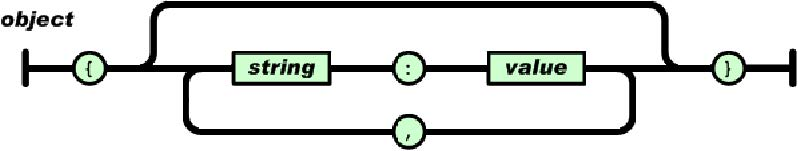
\includegraphics[width=\linewidth]{Images/object_structure.jpg}
		\caption{Object structure}
		\label{fig:object_structure}
	\end{figure}
	
	\begin{figure}
		\centering
		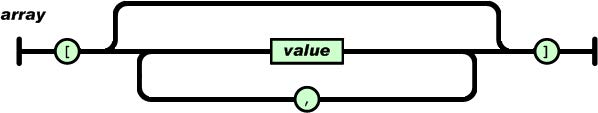
\includegraphics[width=\linewidth]{Images/array_structure.jpg}
		\caption{Array structure}
		\label{fig:array_structure}
	\end{figure}
	
	JSON supports the following data types (see figure \ref{fig:data_types}):
	\begin{itemize}
		\item \textbf{string} (bounded by double quotes)
		\item \textbf{number}
		\item \textbf{object}
		\item \textbf{array}
		\item \textbf{boolean} (true/false)
		\item \textbf{null}
	\end{itemize}
	
	\begin{figure}
		\centering
		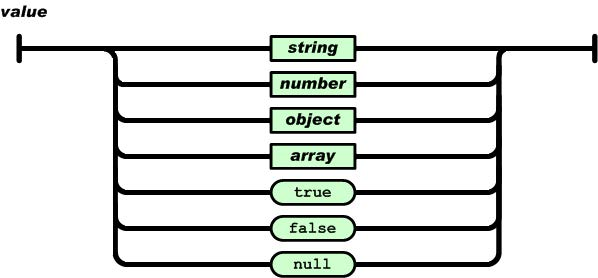
\includegraphics[width=\linewidth]{Images/data_types.jpg}
		\caption{Data types}
		\label{fig:data_types}
	\end{figure}
	
	To transmit these structures, developers must utilize \textbf{serialization} via the \texttt{JSON.stringify} method to convert objects into strings.
	
	\begin{lstlisting}
		let myJSONText = JSON.stringify(myObject);
	\end{lstlisting}
	
	Upon receipt, \textbf{deserialization} via \texttt{JSON.parse} is necessary to reconstruct the functional object.
	
	\begin{lstlisting}
		let myObject = JSON.parse(myJSONtext);
	\end{lstlisting}
	
	The following nested JSON structure illustrates the representation of hierarchical data:
	
	\begin{lstlisting}
	{
	  "glossary": {
	    "title": "example glossary",
	    "GlossDiv": {
	      "title": "S",
	      "GlossList": {
	        "GlossEntry": {
	          "ID": "SGML",
	          "SortAs": "SGML",
	          "GlossTerm": "Standard Generalized Markup Language",
	          "Acronym": "SGML",
	          "Abbrev": "ISO 8879:1986",
	          "GlossDef": {
	            "para": "A meta-markup language, used to create markup
	            languages such as DocBook.",
	            "GlossSeeAlso": ["GML", "XML"]
	          },
	          "GlossSee": "markup"
	        }
	      }
	    }
	  }
	}
	\end{lstlisting}
	
	The environment responsible for processing these data formats is the web browser, which utilizes specialized object models to interface with the user and the document.
	
	\section{JSON serialization, field order and unsupported values}
	
	Let us consider the following code:
	
	\begin{lstlisting}
		function print_name() {console.log(this.name)}
		
		let example_obj = {
			"name": "Davide",
			"surname": "Loconte",
			"id": 590095,
			
			// Nested object
			"address": {
				"city": "Bari",
				"CAP": 70125
			},
			
			/*
				If we use an array the order
				of the values is preserved.
			*/
			"subjects": ["web", "cs", "ai"],
			
			// We can associate a function reference to a key
			"print_name": print_name
		}
		
		console.log(JSON.stringify(example_obj));
	\end{lstlisting}
	
	In this code we define a function and a JavaScript object and then we print a stringified version of the latter. The output is as follows:\\
	
	\{"name":"Davide","surname":"Loconte","id":590095,
	"address":{"city":"Bari","CAP":70125},\\
	"subjects":["web","cs","ai"]\}\\
	
	We can notice that the key \texttt{"print\_name"} is absent because its value is a function reference. JSON was made for data interchange, not code interchange. JSON supports only serializable data meaning that functions, \texttt{undefined} and symbols are ignored during the stringification process. Not to mention the fact that, even if the function body was transferred to another machine, it wouldn't be granted that the receiving application can execute the received code because the receiving application might be written in a different language.\\
	
	As for the order of the fields in the serialized string, theoretically it can change according to the implementation of the serializer and deserializer because JSON is made to define objects as an unordered set of key-value pairs. For the arrays, instead, the order of the values is preserved.\\
	
	In modern JavaScript engine implementations the order of the fields is predictable because it follows the following rules:
	\begin{itemize}
		\item integer-like keys (strings representing integers) $\rightarrow$ ascending order
		\item string keys $\rightarrow$ insertion order order
	\end{itemize}
	
	\chapter{Web API}
	
	The Web API in JavaScript provides a set of interfaces that allow interaction with the browser environment, enabling dynamic web content.
	
	\section{The Browser Environment: BOM and DOM Architectures}
	
	The browser operates on a dual-model architecture that serves as the foundation for web intelligence. This architecture distinguishes between the \textbf{Browser Object Model (BOM)}, representing the host environment, and the \textbf{Document Object Model (DOM)}, representing the specific content.
	
	\subsection{The Browser Object Model (BOM)}
	
	The BOM is centered on the \texttt{window} object, the global entity in the browser environment. It controls features beyond the document content, such as dialogs (\texttt{alert}, \texttt{confirm}), window management (\texttt{close}, \texttt{open}), event handlers, and navigation (\texttt{history}). The \texttt{window.location} property is critical for URL management and provides the following distinct properties:
	
	\begin{itemize}
	    \item \textbf{hash:} The fragment identifier within the URL.
	    \item \textbf{hostname:} The server's domain name or IP address.
	    \item \textbf{port:} The communication port number (e.g., 80 or 443).
	    \item \textbf{pathname:} The path to the specific resource on the server.
	    \item \textbf{protocol:} The communication protocol used (e.g., HTTP or HTTPS).
	    \item \textbf{search:} The query string containing parameters.
	\end{itemize}
	
	The history read-only property returns a reference to the History object, which provides an interface for consulting and manipulating the browser session history (pages visited in the tab or frame that the current page is loaded in). Using this interface it is possible to get the length of the tab history (\texttt{history.length}) and navigate through it using the following functions:
	
	\begin{itemize}
		\item \textbf{back():} This asynchronous method goes to the previous page in session history, the same action as when the user clicks the browser's \textbf{Back} button. Equivalent to \texttt{history.go(-1)}.
		
		\item \textbf{forward():} This asynchronous method goes to the next page in session history, the same action as when the user clicks the browser's \textbf{Forward} button; this is equivalent to \texttt{history.go(1)}. Calling this method to go forward beyond the most recent page in the session history has no effect and doesn't raise an exception.
		
		\item \textbf{go(int):} Asynchronously loads a page from the session history, identified by its relative location to the current page, for example -1 for the previous page or 1 for the next page. If you specify an out-of-bounds value (for instance, specifying -1 when there are no previously-visited pages in the session history), this method silently has no effect. Calling \texttt{go()} without parameters or a value of 0 reloads the current page.
	\end{itemize}
	
	\subsubsection{Example of BOM usage}
	
	In the following code we will expose two common usages of the BOM.
	
	\begin{lstlisting}
	<html>
	  <head>
		<script>
		alert(
		`This is an alert. Use it to inform the
		user of something important.`
		);
		</script>
	  </head>
		
	  <body>
		<h1 id="label">Hello world!</h1>
			
		<script>
		let element = document.getElementById("label");
		confirm(
		`This is a confirm. Use it to ask the user for 
		confirmations and permissions.\n For example: 
		Will you remember that scripts at the bottom of the body
		can access elements in the page even if it hasn't 
		been shown yet? The value of the text you will see in 
		the page is: ${element.innerHTML}`
		);
		</script>
	  </body>
	</html>
	\end{lstlisting}
	
	The first common usage of the BOM is the \texttt{alert} command. This command generates a text box containing a message the user can acknowledge. Use it to inform the user of something important.\\
	
	The second common usage is the \texttt{confirm} command. This command generates a text box with two buttons that make the user decide whether to confirm or refuse an operation. Unlike the \texttt{alert} command which returns \texttt{undefined}, the \texttt{confirm} command can return the following boolean values:
	\begin{itemize}[itemsep=1pt, parsep=1pt, topsep=4pt]
		\item Ok $\rightarrow$ \texttt{true}
		\item Cancel $\rightarrow$ \texttt{false}
	\end{itemize}
	
	Another important thing to notice about the script at the end is the difference between adding an element to the DOM and rendering (painting) it on the screen. An element is added to the DOM as soon as it is parsed, while it is rendered (painted) on the screen later in the rendering process.
	
	\subsection{The Document Object Model (DOM)}
	
	The DOM is the logical tree structure of an HTML document. It defines the hierarchical relationship between elements and provides the \texttt{document} variable as the primary entry point for JavaScript interaction. By treating the document as a tree of nodes, JavaScript can dynamically manipulate styles, attributes, and content via specific methods because each element of an HTML document implements the DOM element interface.\\
	
	Here is an example of a simple HTML document and its relative DOM tree (figure \ref{fig:dom}).
	
	\begin{lstlisting}
		<!DOCTYPE html>
		<html>
			<head>
				<meta charset="UTF-8">
				<title>Example Page</title>
			</head>
			
			<body>
				<h1>DOM tree</h1>
				<p>Hello!</p>
			</body>
		</html>
	\end{lstlisting}
	
	\begin{figure}
		\centering
		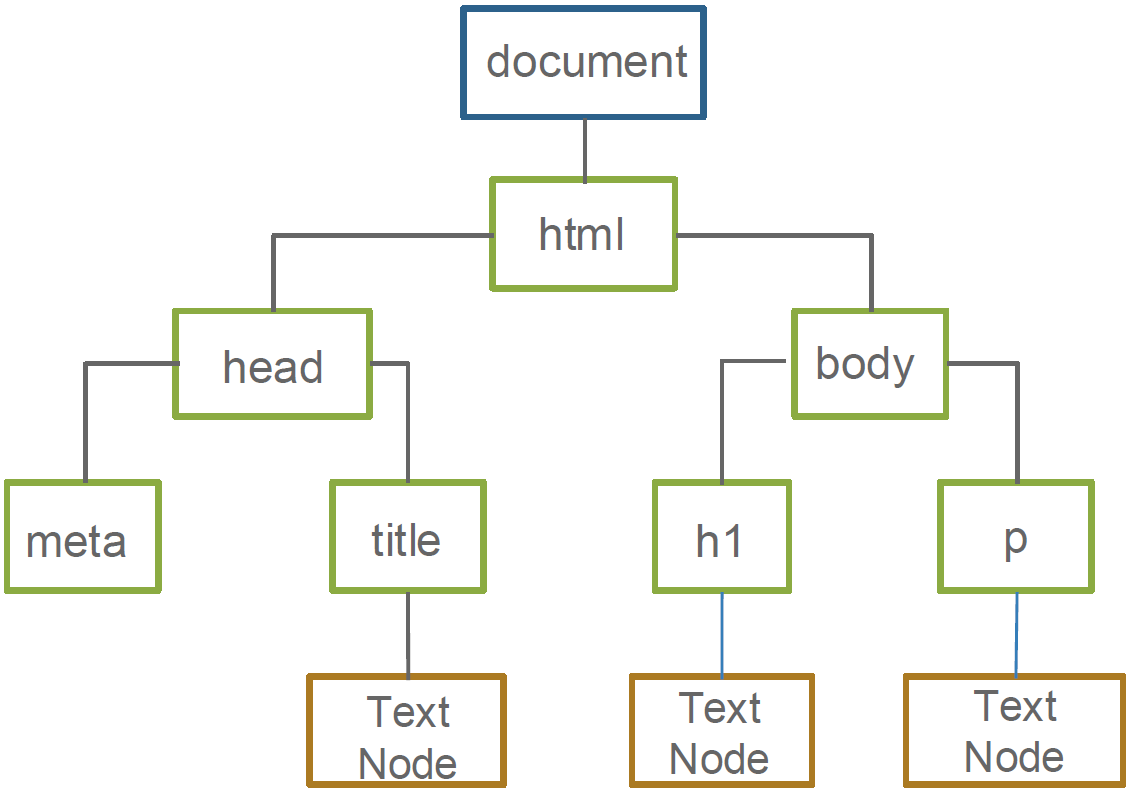
\includegraphics[width=0.5\linewidth]{Images/DOM.png}
		\caption{Document Object Model of the simple HTML document}
		\label{fig:dom}
	\end{figure}
	
	\section{The Document Object: Attributes and Methods}
	
	The \textbf{document} object is a JavaScript object that provides the access to all elements of an HTML document. When the HTML document is loaded in the web browser, it creates a \textbf{document} object. It is the root of the HTML document.\\
	
	The \textbf{document} object contains the various properties and methods you can use to get details about HTML elements and customize them.\\
	
	The JavaScript \textbf{document} object is a property of the \texttt{window} object. It can be accessed using \texttt{window.document} syntax. It can also be accessed without prefixing \texttt{window} object.
	
	\subsection{Document Attributes}
	
	The \texttt{document} object provides several attributes that allow access to collections of elements within an HTML page. These attributes often return arrays (or array-like structures) containing elements in the order they appear in the document.\\
	
	Some common attributes include:
	
	\begin{itemize}
		\item \texttt{document.embeds}: contains all embedded objects in the document;
		
		\item \texttt{document.forms}: contains all the forms defined in the page;
		
		\item \texttt{document.images}: contains all the images present in the document;
		
		\item \texttt{document.links}: contains all the hyperlinks.
	\end{itemize}
	
	Each of these collections can be accessed either by index or by identifier. For example:
	
	\begin{lstlisting}
	document.forms[0];            // access by position
	document.forms["FirstForm"];  // access by id
	\end{lstlisting}
	
	Another important attribute is \texttt{document.body}, which represents the body of the HTML document. It can be manipulated like any other DOM node through the standard element interface.\\
	
	Additional useful attributes include:
	
	\begin{itemize}
		\item \texttt{document.cookie}: allows reading and modifying cookies;
		
		\item \texttt{document.lastModified}: returns the last modification date of the document;
		
		\item \texttt{document.referrer}: indicates the URL of the referring page;
		
		\item \texttt{document.title}: represents the title of the document;
		
		\item \texttt{document.URL}: contains the full URL of the document.
	\end{itemize}
	
	\subsection{Document Methods}
	
	The \texttt{document} object also provides several methods for selecting and creating elements within the DOM.
	
	\subsubsection{Selecting Elements}
	
	\begin{itemize}
		\item \texttt{getElementById("identifier")}: selects an element using its unique identifier.
		
		\item \texttt{querySelector("cssSelector")}: returns the first element that matches a given CSS selector.
		
		\item \texttt{querySelectorAll("cssSelector")}: returns all elements matching the CSS selector as a list of nodes.
	\end{itemize}
	
	Example:
	
	\begin{lstlisting}
	const list = document.querySelector(".list");
	\end{lstlisting}
	
	\subsubsection{Creating Elements}
	
	\begin{itemize}
		\item \texttt{document.createElement("tag")}: creates a new element that can later be inserted into the DOM using standard node manipulation methods.
	\end{itemize}
	
	These methods provide the foundation for dynamically interacting with and modifying the structure of a web page.
	
	\subsection{Event Handlers}
	
	User interaction is mediated by event handlers that trigger functions in response to specific triggers:
	
	\begin{table}[!h]
	\centering
	\begin{tabular}{|l|l|p{8cm}|}
	\hline
	\textbf{Event Type} & \textbf{HTML Attribute} & \textbf{Trigger Description} \\
	\hline
	Blur     & \texttt{onBlur}    & Loss of focus of an element. Blur is the opposite of focus. \\
	\hline
	Change     & \texttt{onChange}    & Modification of a text field, area, or selection list value. \\
	\hline
	Click      & \texttt{onClick}     & User activation of a specific page element. \\
	\hline
	Focus      & \texttt{onFocus}     & Highlighting or selection of a form element for input. \\
	\hline
	Load       & \texttt{onLoad}      & Successful completion of document or resource loading. \\
	\hline
	MouseOver  & \texttt{onMouseOver} & Pointer enters the bounding box of an element. \\
	\hline
	MouseOut   & \texttt{onMouseOut}  & Pointer exits the bounding box of an element. \\
	\hline
	Select     & \texttt{onSelect}    & Selection of text within a form input or text area. \\
	\hline
	Submit     & \texttt{onSubmit}    & Submission of a form to the server. \\
	\hline
	Unload     & \texttt{onUnload}    & The current document is closed or replaced by a new one. \\
	\hline
	\end{tabular}
	\end{table}
	
	For JavaScript to interact with these models effectively, the timing of script execution must be strictly managed to avoid blocking the document parser.
	
	\subsection{Example of DOM manipulation and event handling}
	
	The following example shows how to manipulate the DOM and handle events.
	
	\begin{lstlisting}
<!DOCTYPE html>
<html>
  <body>
	  <h1 id="main_text">Hello world!</h1>
			
	  <script>
		  let div = document.createElement("div");
		  div.append("Text added later");
				
		  document.body.append(div);
				
		  /*
		  We can add an onclick function to an element
		  by adding the 'onclick' attribute.
		  */
		  div.setAttribute('onclick',
		  "alert(\'This functionality was implemented by " +
		  "adding the onclick attribute.\')");
				
		  // Alternatively, we can also add an event listener
		  let main_text = document.getElementById("main_text");
		  main_text.addEventListener("click", function(){
		  	alert("This functionality was implemented by " +
		  	"adding an event listener.");
		  });
	  </script>
  </body>
</html>
	\end{lstlisting}
	
	In this example, the body initially contains only a \texttt{Hello world!} message with an id that allows us to reference it later.\\
	
	The script then creates a new \texttt{div} element and inserts text into it using the \texttt{append} method, which creates a text node. The element is then added to the document by appending it to the \texttt{body}.\\
	
	After that, we define event handlers for user interactions. For the dynamically created \texttt{div}, the click handler is assigned by setting the \texttt{onclick} attribute, although this approach is generally discouraged. For the main text, the event is handled using the \texttt{addEventListener} method, which is the preferred approach.
	
	\section{The Element Interface: Attributes and Methods}
	
	\textbf{Element} is the most general base class from which all element objects (i.e., objects that represent elements) in a \textbf{Document} inherit. It only has methods and properties common to all kinds of elements. More specific classes inherit from \textbf{Element}.\\
	
	For example, the \textbf{HTMLElement} interface is the base interface for HTML elements. Similarly, the \textbf{SVGElement} interface is the basis for all SVG elements, and the \textbf{MathMLElement} interface is the base interface for MathML elements.
	
	\subsection{Element attributes}
	
	The Element interface also exposes attributes that allow direct access to content and styling.
	
	\begin{itemize}
		\item \texttt{element.innerHTML}: allows reading or modifying the HTML content inside the element. This enables dynamic updates of the page structure.
		
		For example:
		
		\begin{lstlisting}
		let div = document.getElementById("container");
		div.innerHTML = "<p>Hello!</p>";
		\end{lstlisting}
		
		\item \texttt{element.style}: returns an object representing the inline CSS styles of the element. Each CSS property is accessible as a corresponding property of this object, allowing dynamic changes to the element's appearance.
		
		For example:
		
		\begin{lstlisting}
		el.style.marginTop = "20px";
		\end{lstlisting}
	\end{itemize}
	
	Through these attributes and methods, developers can dynamically modify both the structure and the presentation of web pages.
	
	\subsection{Element methods}
	
	The Element interface provides several methods to navigate and manipulate the DOM subtree rooted at a specific element.
	
	\begin{itemize}
		\item \texttt{element.getElementsByTagName("tag")}: returns a collection of all descendant elements with the specified tag name within the subtree of the current element;
		
		For example:
		
		\begin{lstlisting}
		/*
			Retrieve all the anchor elements
			nested in the 'el' element.
		*/
		anchorTags = el.getElementsByTagName("a");
		\end{lstlisting}
		
		\item \texttt{element.getAttribute(attributeName)}: retrieves the value of a given attribute of the element;
		
		\item \texttt{element.setAttribute(name, value)}: sets or updates the value of a specified attribute;
		
		\item \texttt{element.appendChild(child)}: adds a new child node at the end of the list of children of the element;
		
		For example:
		
		\begin{lstlisting}
		/*
			Create a paragraph and append it
			to the 'el' element.
		*/
		let p = document.createElement("p");
		el.appendChild(p);
		\end{lstlisting}
	
		\item \texttt{insertBefore(newNode, referenceNode)}: inserts a node before a specified child;
		
		\item \texttt{replaceChild(newNode, oldNode)}: replaces an existing child node;
		
		\item \texttt{removeChild(child)}: removes a child node.
	\end{itemize}
	
	\chapter{Optimized Resource Execution: Script Loading Strategies}
	
	Traditional \texttt{<script>} tags are ``parser-blocking.'' When the browser encounters a script, it halts DOM construction to download and execute it. Placing scripts in the \texttt{<head>} or middle of the document can prevent access to elements located further down the page and create rendering bottlenecks.\\
	
	Modern architecture resolves this using \texttt{async} and \texttt{defer} attributes:
	
	\begin{table}[h]
	\centering
	\begin{tabular}{|l|p{5cm}|p{5cm}|}
	\hline
	\textbf{Feature} & \textbf{\texttt{async}} & \textbf{\texttt{defer}} \\
	\hline
	Download Timing   & Parallel with HTML parsing. & Parallel with HTML parsing. \\
	\hline
	Execution Timing  & Immediately after download, interrupting parsing. & After parsing is complete, but before \texttt{DOMContentLoaded}. \\
	\hline
	Order Maintenance & No. Executes as soon as downloaded. & Yes. Follows the order of appearance in the document. \\
	\hline
	\end{tabular}
	\end{table}
	
	The \texttt{async} attribute is suitable for independent scripts (e.g., analytics) but presents ``race condition'' risks for dependent modules. \texttt{defer} is the preferred standard for scripts requiring a fully constructed DOM. Notably, scripts created dynamically via \texttt{document.createElement} default to \texttt{async}. To ensure these scripts execute in their original document order, the property must be explicitly set: \texttt{script.async = false}.\\
	
	Figure \ref{fig:script_handling_modes} depicts the interaction between HTML parsing and script download and execution in the cases in which the script is handled normally or when the script has the \texttt{async} and \texttt{defer} attributes.
	
	\begin{figure}
		\centering
		
\includegraphics[width=\linewidth]{"Images/normal vs async vs defer.png"}
		\caption{Interaction between the HTML parsing and the JavaScript script in the different handling modes}
		\label{fig:script_handling_modes}
	\end{figure}
	
	\chapter{Other key Web APIs}
	
	\section{Client-Side Persistence: Web Storage vs.\ Cookies}
	
	A shift from server-managed state to client-side persistence allows modern applications to retain user data without excessive network overhead. Web Storage APIs---\texttt{localStorage} and \texttt{sessionStorage}---provide persistent and temporary mechanisms governed by the Same-Origin Policy (matching protocol, domain, and port).
	
	\begin{itemize}
	    \item \textbf{localStorage:} Data is stored on disk and persists across browser restarts until cleared.
	    \item \textbf{sessionStorage:} Data is stored in RAM and is limited to the lifetime of the specific tab.
	\end{itemize}
	
	\textbf{localStorage} is generally used to store user preferences across sessions i.e. the website theme:
	
	\begin{lstlisting}
	// In one session we can set the theme
	localStorage.setItem("theme", "dark");
		
	// In another session we can retrieve the theme
	let theme = localStorage.getItem("theme"); // Dark
	\end{lstlisting}
	
	\textbf{sessionStorage} is used for temporary data like form inputs or login states within a single session:
	
	\begin{lstlisting}
	// We can set the user value after a successful login
	sessionStorage.setItem("user", "davide");
		
	// We can retrieve it later
	let user = sessionStorage.getItem("user"); // davide
	\end{lstlisting}
	
	\subsection{Comparison: Web Storage vs.\ Cookies}
	
	\begin{table}[h]
	\centering
	\begin{tabular}{|l|p{5cm}|p{5cm}|}
	\hline
	\textbf{Feature} & \textbf{Cookies} & \textbf{Web Storage (\texttt{localStorage} and \texttt{sessionStorage})} \\
	\hline
	Size Limit          & 4 KB & \textbf{5 MB} \\
	\hline
	Data Type           & Strings only & Serialized strings (typically JSON objects) \\
	\hline
	Server Transmission & Sent automatically with every HTTP request. & Never sent to the server automatically. \\
	\hline
	Security            & Supports \texttt{HttpOnly} to mitigate XSS (Cross-Site Scripting, a form of malicious code injection attack). & Accessible via JS; vulnerable to XSS. \\
	\hline
	Scope               & Can be shared across subdomains if configured. & Strictly limited to the specific domain. \\
	\hline
	\end{tabular}
	\caption{Comparison of cookies and local storage}
	\label{tbl:cookies_local_storage_comparison}
	\end{table}
	
	Table \ref{tbl:cookies_local_storage_comparison} contains the comparison between cookies and local storage.\\
	
	While Web Storage offers significantly higher capacity, cookies remain essential for authentication because the server can read session IDs directly during the HTTP request lifecycle.
	
	\section{Geolocation API}
	
	The Geolocation API further extends browser intelligence by providing location data. Precision varies by hardware: GPS-enabled mobile devices offer high accuracy, whereas desktop systems fall back to less precise IP-based lookups.
	
	\begin{itemize}
		\item \textbf{getCurrentPosition():} Retrieves the current location of the user
		
		\item \textbf{watchPosition():} Tracks and updates the user’s location as it changes
	\end{itemize}
	
	It is also possible to get the user latitude and longitude using the \textbf{getCurrentPosition()} API as follows:
	
	\begin{lstlisting}
	navigator.geolocation.getCurrentPosition(
	  (position) => {
		  console.log("Latitude:", position.coords.latitude);
		  console.log("Longitude:", position.coords.longitude);
	  }
	);
	\end{lstlisting}
	
	Regardless of precision, these APIs are restricted to secure contexts or remote websites to prevent unauthorized tracking from local files. In fact, using these APIs require explicit user permission and they are also governed by a Same-Origin Policy.
	
	\chapter{Asynchronous JavaScript (AJAX) and Network Interaction}
	
	\textbf{AJAX} is an architectural approach that enables the Single Page Application (SPA) model. Unlike the traditional Wikipedia-style model where every link triggers a full page refresh, AJAX uses an ``AJAX Engine'' (JavaScript) to fetch data in the background and update the DOM dynamically, as seen in applications like Instagram.
	
	\section{Synchronous requests vs asynchronous requests}
	
	\begin{figure}
		\centering
		
\includegraphics[width=\linewidth]{"Images/Synchronous request.jpg"}
		\caption{Synchronous request}
		\label{fig:synchronous_request}
	\end{figure}
	
	In the traditional Wikipedia-style model requests are synchronous. This means that the \textbf{process cycle} is as follows (see figure \ref{fig:synchronous_request}):
	
	\begin{enumerate}
		\item The client sends the request to the server;
		
		\item The client waits for the server to process and return the response;
		
		\item The server sends the response to the client.
	\end{enumerate}
	
	\begin{figure}
		\centering
		
\includegraphics[width=\linewidth]{"Images/Asynchronous request.jpg"}
		\caption{Asynchronous request}
		\label{fig:asynchronous_request}
	\end{figure}
	
	The AJAX model of a web application enables the client to send multiple \textbf{independent} requests to the server without reloading the page. In this model, the \textbf{process cycle} is different and the client interacts with the server through the AJAX engine which acts an intermediary (see figure \ref{fig:asynchronous_request}) and the user is unaware of the underlying process.\\
	
	On the one hand, AJAX has great advantages like:
	\begin{itemize}
		\item Compatibility with the most popular browsers;
		
		\item It makes web pages more interactive and usable to the eyes of the users;
		
		\item Makes serving resources more efficient: the server does not need to transfer the whole web page for each interaction, it only needs to transfer the necessary data.
	\end{itemize}
	
	On the other hand, advanced AJAX implementations introduce specific non-functional challenges regarding state management and system robustness because, as highlighted in the figure, there isn't a strict order among the operations in the process cycle. Notice that right before the first server transmission to the AJAX engine, the latter displays something to the user. It may seem like the AJAX engine can show data to the user before receiving it but it can't because it's physically impossible. Instead, the information you see displayed to the user is the response of a previous request to the server.\\
	
	The following subsections expose how to address these issues.
	
	\subsection{Race Conditions in Search Inputs}
	
	A classic architectural bug occurs when a user types into a live-search bar. If a user types ``cat'' quickly, the browser sends requests for ``c'', ``ca'', and ``cat''. Because \textbf{independent} asynchronous responses do not guarantee order, the response for the first letter (``c'') might arrive after the response for the full word (``cat''), causing the UI to display the wrong results. Solutions include:
	
	\begin{enumerate}
		\item \textbf{Debouncing:} Delaying the request until the user pauses typing.
		\item \textbf{Request Cancellation:} Using \texttt{AbortController} to cancel previous unfinished requests.
		\item \textbf{Versioning:} Tagging requests with IDs and ignoring any response that is not the most recent.
	\end{enumerate}
	
	These technique are used by high quality search bars like the one by Google to make sure that the user only receives the right responses.
	
	\newpage
	\subsection{SEO and User Experience}
	
	AJAX-heavy sites break the traditional ``one page = one URL'' model. This interferes with \textbf{Search Engine Indexing}, as crawlers primarily read initial HTML, and breaks \textbf{Bookmark/History Management}. If a user clicks the ``Back'' button, the browser might navigate away from the site entirely rather than reverting an AJAX-driven state change.\\
	
	\textbf{Standard Solutions:}
	
	\begin{itemize}
		\item \textbf{History API:} The industry standard for programmatically updating the URL and browser history without a page refresh, ensuring that ``Back/Forward'' navigation and bookmarks work as expected.
		
		\item \textbf{Server-Side Rendering (SSR):} Executing JavaScript on the server to provide a complete HTML document to search engine crawlers.
	\end{itemize}
	
	\section{AJAX endpoints as attack surfaces and security considerations}
	
	AJAX endpoints represent a fundamental component of modern web applications, enabling asynchronous communication between client and server. However, from a security perspective, they also constitute critical access points that can be exploited by malicious users.
	
	\subsection{AJAX endpoints as vulnerability points}
	
	Every AJAX request targets a server-side endpoint that processes input and returns data. These endpoints are often exposed over HTTP and can be invoked programmatically, making them attractive targets for attackers.\\
	
	Malicious users may exploit AJAX endpoints in several ways:
	
	\begin{itemize}
		\item \textbf{Denial of Service (DoS):} by issuing a large number of asynchronous requests, attackers can overwhelm the server, exhausting computational or network resources.
		
		\item \textbf{Unauthorized Data Access:} if endpoints lack proper authentication or authorization checks, attackers may retrieve sensitive information.
		
		\item \textbf{Injection Attacks:} improperly validated input sent via AJAX can lead to SQL injection, command injection, or other forms of exploitation.
		
		\item \textbf{Automation of Attacks:} since AJAX calls are easily reproducible, attackers can script repeated requests to systematically probe the system.
	\end{itemize}
	
	These characteristics make AJAX endpoints a significant part of the application's attack surface.
	
	\subsection{Same-Origin Policy and CORS}
	
	A first line of defense in web security is the \textit{Same-Origin Policy}, which prevents browsers from making requests to a different origin (defined by protocol, domain, and port) unless explicitly allowed.\\
	
	To enable controlled cross-origin interactions, servers can adopt \textit{Cross-Origin Resource Sharing (CORS)}. This mechanism relies on specific HTTP headers:
	
	\begin{itemize}
		\item \texttt{Access-Control-Allow-Origin}: defines which origins are allowed to access the resource.
		\item \texttt{Access-Control-Allow-Methods}: specifies permitted HTTP methods (e.g., GET, POST).
		\item \texttt{Access-Control-Allow-Headers}: lists allowed request headers.
		\item \texttt{Access-Control-Allow-Credentials}: indicates whether cookies can be included.
	\end{itemize}
	
	Additionally, browsers distinguish between \textit{simple requests} (e.g., basic GET requests) and \textit{preflight requests}, where an initial \texttt{OPTIONS} request is sent to verify permissions before executing more complex operations.\\
	
	While CORS provides flexibility, misconfiguration (e.g., allowing all origins with \texttt{*}) can expose endpoints to unauthorized access.
	
	\subsection{Defense Mechanisms}
	
	To mitigate risks associated with AJAX endpoints, several defensive strategies should be adopted:
	
	\begin{itemize}
		\item \textbf{Authentication and Authorization:} ensure that every endpoint verifies user identity and permissions;
		
		\item \textbf{Rate Limiting:} limit the number of requests per client to prevent DoS attacks;
		
		\item \textbf{Input Validation and Sanitization:} validate all incoming data to prevent injection attacks;
		
		\item \textbf{Secure CORS Configuration:} restrict allowed origins and methods to only trusted ones;
		
		\item \textbf{Use of Tokens (e.g., CSRF Tokens):} protect endpoints from cross-site request forgery attacks.
	\end{itemize}
	
	\subsection{Example of a Complete CORS Header Configuration}
	
	The following example shows a possible HTTP response header configuration that includes all the main CORS directives discussed previously:
	
	\begin{lstlisting}
	HTTP/1.1 200 OK
	Content-Type: application/json
		
	Access-Control-Allow-Origin: https://example.com
	Access-Control-Allow-Methods: GET, POST, PUT, DELETE
	Access-Control-Allow-Headers: Content-Type, Authorization
	Access-Control-Allow-Credentials: true
	\end{lstlisting}
	
	In this configuration:
	
	\begin{itemize}
		\item \texttt{Access-Control-Allow-Origin} restricts access to a specific trusted domain;
		
		\item \texttt{Access-Control-Allow-Methods} explicitly lists the allowed HTTP methods;
		
		\item \texttt{Access-Control-Allow-Headers} defines which custom headers can be used in requests;
		
		\item \texttt{Access-Control-Allow-Credentials} enables the inclusion of cookies and authentication data.
	\end{itemize}
	
	For completeness, a preflight response (to an \texttt{OPTIONS} request) may include the same headers:
	
	\begin{lstlisting}
	HTTP/1.1 204 No Content
		
	Access-Control-Allow-Origin: https://example.com
	Access-Control-Allow-Methods: GET, POST, PUT, DELETE
	Access-Control-Allow-Headers: Content-Type, Authorization
	Access-Control-Allow-Credentials: true
	\end{lstlisting}
	
	This configuration ensures controlled cross-origin access while maintaining a secure policy by limiting interactions to trusted clients.\\
	
	In summary, AJAX endpoints significantly enhance interactivity but also introduce security risks. The Same-Origin Policy and CORS mechanisms help regulate cross-origin access, but they must be carefully configured. A secure design requires combining browser-level protections with robust server-side controls to reduce the exposure of these endpoints to malicious exploitation.
	
	\section{The \texttt{XMLHttpRequest} (XHR) and the Fetch API}
	
	The \texttt{XMLHttpRequest} (XHR) object is the traditional mechanism used to perform AJAX requests. It provides fine-grained control over HTTP communication, but requires a more verbose and event-driven programming style.
	
	\subsection{XHR Lifecycle and readyState property}
	
	An XHR request evolves through different states, tracked by the \texttt{readyState} property:
	
	\begin{itemize}
		\item \textbf{0 (UNSENT):} object created, but \texttt{open()} not yet called;
		
		\item \textbf{1 (OPENED):} \texttt{open()} has been called;
		
		\item \textbf{2 (HEADERS\_RECEIVED):} \texttt{send()} has been called, response headers are available;
		
		\item \textbf{3 (LOADING):} response data is being received;
		
		\item \textbf{4 (DONE):} request completed and response fully available.
	\end{itemize}
	
	The \texttt{onreadystatechange} callback is triggered whenever the state changes and is commonly used to handle the response.\\
	
	\subsubsection{XHR request lifecycle example}
	
	This is an example showing how the state changes during the lifecycle of an XHR request.
	
	\begin{lstlisting}
	const xhr = new XMLHttpRequest();
	console.log("UNSENT", xhr.readyState); //readyState 0
	
	xhr.open("GET", "/api", true);
	console.log("OPENED", xhr.readyState); //readyState 1
	
	xhr.onprogress = () => {
		console.log("LOADING", xhr.readyState); //readyState 3
	};
	
	xhr.onload = () => {
		console.log("DONE", xhr.readyState); //readyState 4
	};
	
	xhr.send(null);
	\end{lstlisting}
	
	\subsection{XHR Methods and Execution Flow}
	
	XHRs have the following methods:
	
	\begin{enumerate}
		\item \texttt{open(method, url [, async] [, user] [, password])}: this method initializes the request and has the following arguments:
		\begin{itemize}
			\item \texttt{method}: The HTTP method (GET, POST, PUT, DELETE);
			
			\item \texttt{url}: The URL of the resource to send the request to;
			
			\item \texttt{async}: Optional boolean parameter specifying if the request is synchronous (false) or asynchronous (true, default value);
			
			\item \texttt{user} and \texttt{password}: Optional credentials for authentication purposes. Their default value is \texttt{null}.
		\end{itemize}
		
		\item \texttt{send([data])}: sends the request to the server. The \texttt{data} parameter is optional and is used for POST and PUT requests. Its default value is \texttt{null}.
		
		\item \texttt{setRequestHeader(header, value)}: Sets the value of an HTTP request header, for example to specify the content type of data to be sent to the server.
		It must be called after \texttt{open()} and before \texttt{send()}. \texttt{setRequestHeader(header, value)} does not accept arrays as input, therefore it must be called once for each header. If the same header is set multiple times, its values are typically concatenated into a single header separated by commas, rather than being overwritten.\\
		
		For example:
		
	\begin{lstlisting}
	xhr.setRequestHeader("Content-Type", "application/json");
	xhr.setRequestHeader("X-Auth", "123");
	xhr.setRequestHeader("X-Auth", "456");
	\end{lstlisting}
		
		In this case the header becomes:
		
	\begin{lstlisting}
	Content-Type: application/json
	X-Auth: 123, 456
	\end{lstlisting}
		
		\item \texttt{getAllResponseHeaders()}: Returns a string containing all the response headers separated by a CRLF character;
		
		\item \texttt{getResponseHeader(headerName)}: Returns a string containing the value of the requested header specified using the \texttt{headerName} parameter.
	\end{enumerate}
	
	The typical workflow of an XHR request involves three main steps:
	
	\begin{enumerate}
		\item \textbf{\texttt{open(method, url, async)}};
		
		\item Optionally one or more \textbf{\texttt{setRequestHeader()}};
		
		\item \textbf{\texttt{send(data)}}.
	\end{enumerate}
	
	\subsubsection{Why is \texttt{open()} required before \texttt{send()}?}
	
	The \texttt{open()} method does \textbf{not} establish a network connection or perform a handshake with the server. Instead, it:
	
	\begin{itemize}
		\item configures the request by specifying the HTTP method, target URL, and whether it is asynchronous;
		\item transitions the object from state 0 (UNSENT) to state 1 (OPENED);
		\item prepares the internal request structure so that headers and callbacks can be correctly attached.
	\end{itemize}
	
	The actual network communication starts only when \texttt{send()} is invoked. Therefore:
	
	\begin{itemize}
		\item there is \textbf{no preliminary handshake} triggered by \texttt{open()};
		\item \texttt{open()} is a configuration step, not a connectivity check;
		\item event handlers such as \texttt{onreadystatechange} should be defined before \texttt{send()} to avoid missing state transitions.
	\end{itemize}
	
	\subsection{XHR properties}
	
	In addition to the \texttt{readyState} property, which tracks the lifecycle of a request, the \texttt{XMLHttpRequest} object provides several other useful properties that allow developers to inspect the response and control how data is handled.
	
	\begin{itemize}
		\item \texttt{status}: represents the HTTP status code returned by the server (e.g., 200 for success, 404 for not found, 500 for server error). It is commonly used to determine whether a request has been successfully completed;
		
		\item \texttt{statusText}: a textual description of the HTTP status code (e.g., ``OK'', ``Not Found''). It is mainly useful for debugging and logging purposes;
		
		\item \texttt{responseType}: specifies the expected format of the response. It must be set after calling \texttt{open()} and before calling \texttt{send()}. Possible values include:
		\begin{itemize}
			\item \texttt{"text"}: plain text (default);
			\item \texttt{"json"}: JSON data automatically parsed into a JavaScript object;
			\item \texttt{"document"}: HTML or XML document;
			\item \texttt{"blob"} or \texttt{"arraybuffer"}: binary data.
		\end{itemize}
		
		\item \texttt{response}: contains the response data in a format consistent with the value of \texttt{responseType}. For example, if \texttt{responseType = "json"}, this property contains a JavaScript object;
		
		\item \texttt{responseText}: contains the response as a plain text string. This property is typically used when \texttt{responseType} is \texttt{"text"} or left unspecified;
		
		\item \texttt{responseXML}: contains the response parsed as an XML document. It is valid only when the response is XML or when \texttt{responseType} is set to \texttt{"document"};
		
		\item \texttt{onreadystatechange}: an event handler (callback function) that is invoked every time the \texttt{readyState} property changes.\\
		
		This property is fundamental for handling asynchronous requests, as it allows the developer to monitor the progression of the request and execute code when the operation is completed.\\
		
		A common pattern is to check when the request reaches the \texttt{DONE} state (i.e., \texttt{readyState === 4} or, alternatively, \texttt{xhr.readyState === XMLHttpRequest.DONE} as XHR ready states are enumerated) and then verify the HTTP status:
		
		\begin{lstlisting}
	xhr.onreadystatechange = function() {
	  if(xhr.readyState === XMLHttpRequest.DONE) {
		  const status = xhr.status;
		  if (status === 0 || (status >= 200 && status < 400)) {
			  // the request has been completed successfully
			  console.log(xhr.responseText);
		  } else {
			  // there is some error with the request!
			  console.error(`${xhr.status}: ${xhr.statusText}`)
		  }
	  }
	};
		\end{lstlisting}
		
		It is important to define \texttt{onreadystatechange} before calling \texttt{send()}, otherwise some state transitions might not be captured.\\
		
		Modern alternatives to this handler include \texttt{onload} (triggered when the request completes successfully) and \texttt{onerror} (triggered in case of network errors).
	\end{itemize}
		
	These properties allow developers to handle different types of responses and to build more robust and flexible AJAX-based applications.
	
	\subsection{Example of XMLHttpRequest}
	
	This is a full example of XHR request to the website \hyperlink{https://jsonplaceholder.typicode.com/}{https://jsonplaceholder.typicode.com/} which provides a free fake and reliable API for testing and prototyping.\\
	
	The reader is encouraged to copy and paste the script in a browser console to check its output for themselves and memorize the example because XHR requests are recurrent when programming JS front-end scripts.
	
	\begin{lstlisting}
	const xhr = new XMLHttpRequest();
		
	// We have to write this function first and then send the request.
	xhr.onreadystatechange = function (response) {
	  /*
		Make sure to check the readyState an remember
		that the ready states are enumeratedas follows:
		  0: UNSENT
		  1: OPENED
		  2: HEADERS_RECEIVED
		  3: LOADING
		  4: DONE
	  */
	  if (xhr.readyState === XMLHttpRequest.HEADERS_RECEIVED){
	  console.log("The headers have been received");
	  console.log("XHR ready state: " + xhr.readyState);
		console.log(xhr);
	  }
			
	  if (xhr.readyState === XMLHttpRequest.LOADING){
		console.log("The response is being loaded");
		console.log("XHR ready state: " + xhr.readyState);
		console.log(xhr);
	  }
			
	  if (xhr.readyState === XMLHttpRequest.DONE){
		console.log("Calling on ready state change");
		console.log("XHR ready state: " + xhr.readyState);
		console.log(xhr);
		console.log(JSON.parse(xhr.response));
	  }
	}
		
	// Now the request is unsent
	console.log("The request is unsent");
	console.log("XHR ready state: " + xhr.readyState);
	console.log(xhr);
		
	xhr.open('GET', 'https://jsonplaceholder.typicode.com/todos/1');
		
	// Now the request is opened
	console.log("The request is opened");
	console.log("XHR ready state: " + xhr.readyState);
	console.log(xhr);
		
	xhr.send();
	\end{lstlisting}
	
	\subsection{Fetch API: A Modern Approach}
	
	The Fetch API provides a modern alternative to XHR, based on Promises rather than event callbacks.\\
	
	Key characteristics:
	
	\begin{itemize}
		\item \textbf{Promise-based model:} asynchronous flows are handled using \texttt{then()} and \texttt{catch()}, improving readability. The following snippet illustrates an example of failing request.
		
		\begin{lstlisting}
	fetch('https://api.example.com/data')
	.then(response => {
	  if (!response.ok) throw new Error('Request failed');
	  return response.json(); // Parse JSON response
	})
	.then(data => console.log(data))
	.catch(error => console.error('Error:', error));
		\end{lstlisting}
		
		This request fails because the URL \texttt{'https://api.example.com/data'} does not exist so, \texttt{response.ok = false}, the error object is thrown and is caught in the last line of the snippet;
		
		\item \textbf{Cleaner syntax:} avoids manual state tracking (\texttt{readyState});
		
		\item \textbf{Built-in JSON handling:} methods like \texttt{response.json()} simplify parsing;
		
		\item \textbf{Flexible configuration:} supports custom HTTP methods, headers, and request bodies. For example, a POST request is as follows:
		
		\begin{lstlisting}
	fetch('https://api.example.com/data', {
	  method: 'POST',
	  headers: { 'Content-Type': 'application/json' },
	  body: JSON.stringify({ key: 'value' })
	});
		\end{lstlisting}
	\end{itemize}
	
	\subsection{Example of request using the fetch API}
	
	Now, let us rewrite the same example as before but using the fetch API.
	
	\begin{lstlisting}
	fetch('https://jsonplaceholder.typicode.com/todos/1')
	.then((response) => {
	  return response.json();
	})
	.then(response => {
	  console.log(response);
	})
	  .catch((response) => {
		console.log("There was an error");
	});
	\end{lstlisting}
	
	\subsection{XHR vs Fetch: Key Differences}
	
	\begin{itemize}
		\item \textbf{Programming model:} XHR is event-driven, Fetch is promise-based;
		
		\item \textbf{Complexity:} XHR requires manual state management, whereas Fetch is more concise.
		XHR provides fine-grained control over the request lifecycle; however, this level of control is not required in most cases. 
		For this reason, the Fetch API was introduced to abstract away explicit state management and simplify asynchronous programming;
		
		\item \textbf{Error handling:} Fetch uses promise rejection, while XHR relies on status checks and event handlers;
		
		\item \textbf{Modern usage:} Fetch is the preferred standard for new applications, while XHR is maintained mainly for backward compatibility.
	\end{itemize}
	
	In summary, XHR offers low-level control over HTTP requests, while Fetch provides a higher-level abstraction that simplifies asynchronous programming.

\end{document}
